% sections/prefetching.tex
% TJ WILL WRITE THIS SECTION !!!

\subsection{Link Prefetching}

Link prefetching is a HTML syntax that gives the web browser a hint about which page the user is most likely to visit in the near future.
For the prefetching resources that a web page specifies, the browser silently loads them after idle time and store them in cache. 
It was first suggested by Mozilla Foundation, and is adopted by most modern browsers nowadays.

Today's web browsers makes use of a specific syntax called \emph{pre-fetching}, which was proposed as a draft standard by Mozilla.
Using pre-fetching, browser can predicts documents likely to be visited by the user in the near future.
Therefore, based on the hint provided by pre-fetching a browser is able to fetch those documents a head of time.
In fact, it is the web page that provides a set of pre-fetching hints for the browser.
Then, loading the page and passing an idle time, the browser starts to pre-fetch and cache specified documents.
Needless to say, this mechanism improves efficiency.
Particularly, it is most effective if the content provider may be reasonably certain which links users are going to visit next \cite{wikiPreF}.

% Insert a figure of "prefetch-network" which shows the network traffic.
% explain about how prefetching actually works 


\subsection{Effects of Prefetching on Fingerprinting}
% cite some papers to describe about the features that are used for attacks,
% and explain why prefetching change the feature.

% Vaibhav says: put the intuition down 

See Figure~\ref{fig:prefetch}. It's not so pretty though.
\begin{figure}[h]
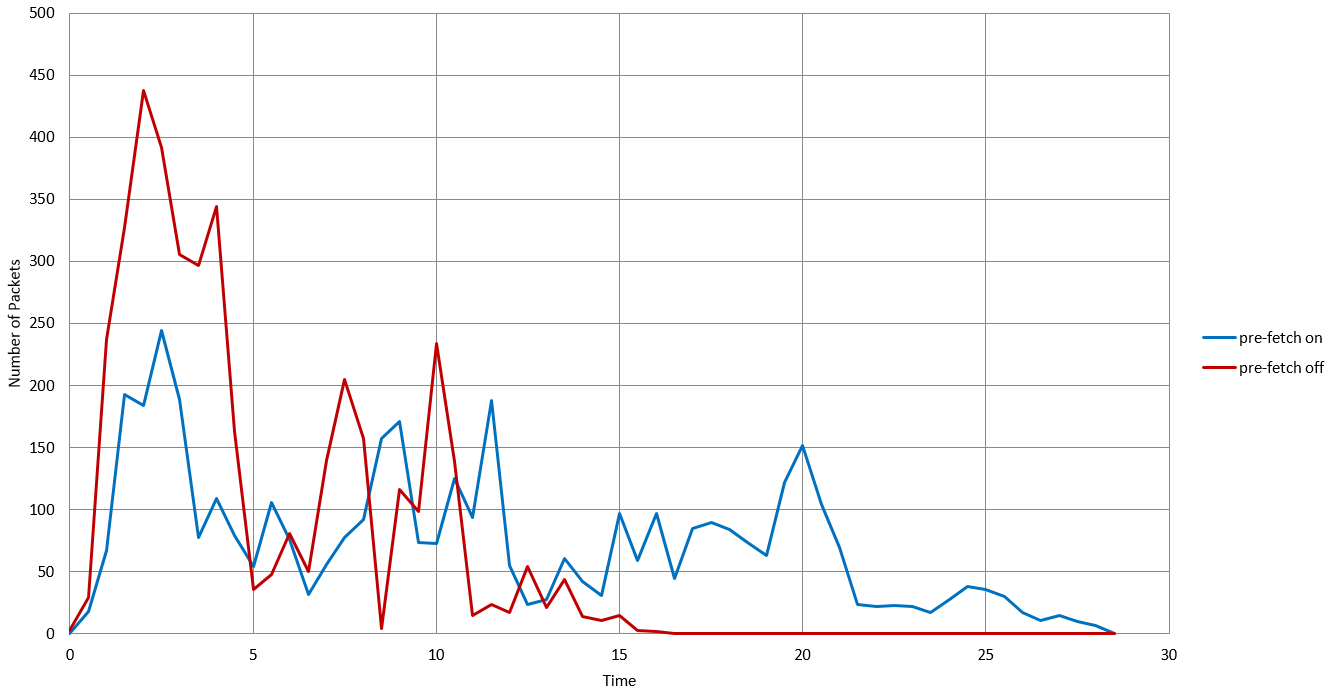
\includegraphics[width=\columnwidth]{figures/prefetch.png}
\centering
\caption{hi}
\label{fig:prefetch}
\end{figure}


